\documentclass[conference]{IEEEtran}
\IEEEoverridecommandlockouts
\usepackage{graphicx}
\usepackage{paralist}
\usepackage{algorithm}
\usepackage{algorithmicx}
\usepackage{algpseudocode}
\usepackage[dvipsnames]{xcolor}
\usepackage{amsmath}
\usepackage{hyperref}
\usepackage{caption}
\usepackage{subcaption}
\usepackage{ulem}
\usepackage{tabularx}

% Fix link colors
\hypersetup{
    colorlinks = true,
    linkcolor=red,
    citecolor=red,
    urlcolor=blue,
    linktocpage % so that page numbers are clickable in toc
}

\algblock{Input}{EndInput}
\algnotext{EndInput}
\algblock{Output}{EndOutput}
\algnotext{EndOutput}
\newcommand{\Desc}[2]{\State \makebox[2em][l]{#1}#2}

\newcommand{\tristan}[1]{\color{orange}\textbf{From Tristan:}#1\color{black}}
\newcommand{\henri}[1]{\color{green}\textbf{From Henri:}#1\color{black}}
\newcommand{\english}[1]{\uwave{#1}}

\newcommand{\valerie}[1]{\color{blue}\textbf{From Valerie:}#1\color{black}}


\begin{document}

%\title{Simulating the Linux page cache in distributed applications with WRENCH}
\title{Simulating the Linux page cache in distributed applications with WRENCH}

\author{
  \IEEEauthorblockN{
    Hoang-Dung Do\IEEEauthorrefmark{1},
    Val\'erie Hayot-Sasson\IEEEauthorrefmark{1},
    Rafael Ferreira da Silva\IEEEauthorrefmark{3},
    Henri Casanova\IEEEauthorrefmark{2},
    Tristan Glatard\IEEEauthorrefmark{1}
  }\\
  \IEEEauthorblockA{
    \IEEEauthorrefmark{1}Department of Computer Science and Software Engineering, Concordia University, Montreal, Canada\\
    \IEEEauthorrefmark{2}Department of Information and Computer Sciences, University of Hawai`i at M\=anoa, USA\\
    \IEEEauthorrefmark{3}Information Sciences Institute, University of Southern California, Marina Del Rey, CA, USA
  }
}

\maketitle

    \begin{abstract}

    % Henri Rewrote quite  a bit in the next paragraph here to spell out a bit
    % more why we need simulation
    The emergence of Big Data in recent years has resulted in a growing
    need for efficient data storage management techniques.  While
    infrastructures with sufficient compute power are available to
    process large datasets, the I/O bottleneck remains.  A
    well-known and ubiquitous approach for reducing the overhead of
    I/O operations is to use the Linux page cache.  It is thus crucial
    to study experimentally the impact of the Linux page cache on the
    performance Big Data applications. Given the difficulties with and shortcomings of
    real-world experiments, a popular approach for application
    performance studies is to use simulation.  While many simulation
    frameworks have been developed for this purpose, they do not 
        simulate page caching fully, or even at all.  As a result, using
    these frameworks for studying the performance of data-intensive
    applications leads inaccurate simulation results. 

        % Some cosmetic rewrites below
    In this paper, we propose a I/O simulation model that characterizes
    the key features of the page cache. We have implemented this model
    as  part of the WRENCH workflow simulation framework, which itself
    builds on the popular SimGrid distributed systems simulation
    framework.  Our model and its implementation enable the simulation
    of both single-threaded and multithreaded applications, and of both
    writeback and writethrough caches for local or network-based
    filesystems. We evaluate the accuracy of our model in different
    conditions, including sequential and concurrent applications, as
    well as local and remote I/Os.  We find that our page cache model
    reduces the simulation error by up to an order of magnitude when
    compared to state-of-the-art, cacheless simulations.

    \end{abstract}

    \section{Introduction}

        The Linux Page Cache plays an important role in
        reducing filesystem data transfer times. With the page cache, previously
        read data can be re-read directly from memory and written data can be written to
        memory before being asynchronously flushed to disk, resulting in improved I/O performance
        on slower storage devices. The magnitude of the performance benefits that can be obtained from using the page
        cache are determined by many factors including the total amount of memory,
        the amount of data being written (i.e., dirty data), and the percentage of available memory available for
        written data. All these factors are important when determining the impact of I/O on
        application performance, particularly in data-intensive applications.

        % Swapped the order the two paragraphs and merged them into one
        The number of data-intensive applications has been steadily rising as a result of
        open-data and data sharing initiatives. Due to the sheer size of the data being
        processed, these applications must be executed on large scale infrastructure
    such as High Performance Computing (HPC) clusters or the cloud.  It
    is thus crucial to quantify the performance of these applications
    on these platforms. The goals include determining which type of hardware/software
    stacks are best suited to different application classes, as well as
    understanding the shortcomings of current algorithms, designs and
    technologies so as to propose new solutions. Unfortunately, application performance
        studies via experiments on real-world compute platforms
        faces several difficulties (high operational costs, labor-intensive experimental setups,
        shared platforms with dynamic loads that hinder reproductibilty of results) and shortcomings
        (experiments are limited to the available platform/softare configurations, which precludes
        the exploration of hypothetical scenarios). 
    Simulations address these concerns by providing simulation models
    and abstractions for the performance of computer hardware, such as
    CPU, network and storage. Consequently, simulations provide a
    cost-effective, fast, easy and reproducible way to evaluate
    application performance on arbitrary platform configurations. It thus comes
        as no surprise that, considering here only the field of parallel and distributed
        computing, a large number of simulation frameworks have been developed and used
        to support research and development endeavors~\cite{LAUNDRYLISTOFREFS_THAT_HENRI_WILL_PUT_IN}.

        Page caching is a well-known and ubiquitous technique for mitigating the I/O bottleneck
        faced by data-intensive applications. As such, it is necessary to simulate page caching
        when performing performance studies in simulation.
        Furthermore, simulating the page cache makes it possible to study relevant application-I/O
        bottlenecks that can arise over the course of execution, such as page cache
        starvation~\cite{zhuang2017}.
        While existing simulation frameworks of parallel and distributed computing
        systems  capture many relevant features of hardware/software stacks of interest, 
        they lack the ability to simulate page caches adequately. Those frameworks
        that implement some page cache simulation
        fail to capture key features such
        as dirty data and cache eviction policies~\cite{nunez2012simcan,nunez2012icancloud}. 
        Some simulators, such as that in~\cite{xu2018saving}, do capture such features,
        but are domain-specific. 

        %However, there is a trade-off between accuracy and scalability, which has been
        %indicated in some reviews \cite{casanova2014simgrid} \cite{byrne2017review}.
        %This means that in most cicumstances, users have to, more or less, sacrifice
        %accuracy for the scalability and performance when their platforms grow to
        %hundreds or thousands nodes.

    In this work, we present WRENCH-cache, a simulation model of I/O
    with page cache incorporated into the WRENCH simulation framework~\cite{casanova2018wrench},
    which is  based on the popular SimGrid distributed simulation framework~\cite{XXX}.
    The added value of WRENCH-cache is to make it possible to simulate 
        application execution accurately in the presence of page caching. Our specific 
        contributions are as follows:
    \begin{compactitem}
        \item A page cache simulation model that supports 
    both single-threaded and multithreaded applications, and of both
    writeback and writethrough caches for local or network-based
    filesystems;
        \item An implementation of this model as part of the WRENCH framework; 
        \item An evaluation and validation of the accuracy of our model, and of its implementation,
              for a range of applications, platforms, and page cache configurations. 
    \end{compactitem}



    \section{Related Work}
    \label{relatedwork}

        \subsection{Page cache}

        To improve performance of disk accesses, the page cache was introduced to the Linux kernel. %It contains pages referring to physical pages on disk \cite{linuxdev3rd2010}.
            The goal of the page cache is to try ensure that most I/O operations occur entirely
            within memory space rather than synchronously to and from the storage device.
            All disk-backed data located in the page cache are partitioned into many small pages.
            When a read operation is initiated, the kernel checks whether the required pages are in memory.
            If it is the case, data is read entirely from memory (i.e. \textit{cache hit}). Otherwise,
            the necessary pages must be loaded to memory from the disk (i.e. \textit{cache miss})
            Conversely, for writing, one of three strategies can be applied: direct~I/O (or, ``no-write''),
            writethrough and writeback.
            If direct~I/O is enabled for a given file system, all I/O operations bypass the
            page cache for writes, writing data directly to disk. In contrast, write-through enables the page cache
            for file system writes, but the data is written synchronously from memory to disk. Writeback extends write-through
            by enabling asynchronous writes to disk, meaning that a write call will return once
            the data has been written to memory.
            The writeback strategy is considered to outperform write-through as well as
            direct I/O as it delays disk writes to perform a bulk write at a later time
            \cite{linuxdev3rd2010}.


            Cache eviction and flushing strategies are integral to proper page cache functioning.
            Whenever space in memory becomes limited, either as a result of application memory
            or page cache use, page cache data may be evicted. Only data that
            has been persisted to storage (clean pages) can be flagged for eviction and removed from
            memory. Written data that has not yet been persisted to disk (dirty data) must first
            be copied (flushed) to storage prior to eviction. When sufficient memory is
            being occupied, the flushing process is synchronous. However, even when
            there is sufficient available memory, written data will be flushed to disk
            at a predefined interval through a process known as \textit{periodical flushing}.
            Periodical flushing only flushes expired dirty pages, which remain dirty in
            page cache longer than an expiration time configured in the kernel.
            Different cache eviction algorithms have also been developed and proposed
            \cite{owda2014comparison}.
            The Linux kernel uses a two-list strategy to flag pages for eviction.
            The two-list strategy is based on a least recently used (LRU) policy
            and uses an active and inactive list in its implementation.
            If accessed pages are not in the page cache, they are added to the inactive list.
            Should pages located on the inactive list be accessed, they will be moved from
            the inactive to the active list.
            The lists are also kept balanced by moving pages from the active list
            to the inactive list when the active list grows too large.
            Thus, the active list only contains pages which are accessed more than once
            and not evictable, while the inactive list includes pages accessed once only,
            or pages that have be accessed more than once but moved from the active list.
            Both lists operate using LRU eviction policies meaning the data that has
            not be accessed recently will be moved first.

        \subsection{Simulators}

            Many simulation frameworks exist to describe the behaviour of applications
            running on the various infrastructures available to users, such as personal computers,
            clouds and clusters.
            These simulators are built with resource models such CPU, network and
            storage, using various different approaches to describe the hardware.
            For example, there is \textit{CloudSim} and \textit{iCanCloud} for packet-level network models
            and \textit{DiskSim} the simulates storage hardware functioning \tristan{add references}.

            Simulators must choose between scalability and accuracy when describing the
            hardware~\cite{casanova2014simgrid}.
            Fine-grained models allow simulators to achieve high accuracy,
            but lead to scalability issues due to long simulation time
            when simulated platforms and applications grow.
            SimGrid is an open source simulation platform that has been developed
            not only to balance the trade-off between accuracy and scalability,
            but also to achieve versatility, allowing the use of the framework
            to simulate applications in multiple domains. WRENCH, a workflow management
            system simulator based on the SimGrid framework, provides a high-level API
            for simulating workflows, thus facilitating the integration of new models.
            \valerie{say more about wrench}

            Despite the fact that many sophisticated models for resources have been
            integrated in simulators, and the page cache shows apparent impacts on I/O
            performance, the simulation model of page cache is still missing in most
            of simulators.
            For example, SimGrid only simulates I/O operations with storage bandwidths
            and capacity.
            SIMCAN is a simulation framework that models page cache by storing data
            accessed on disk in a block cache \cite{nunez2012simcan}.
            Page cache is also modeled in the iCanCloud simulator through a component which
            manages memory accesses and cached data \cite{nunez2012icancloud}. However,
            the scalability of the iCanCloud simulator is limited by its sophisticated model.
            Ultimately, none of these simulators provide any writeback cache simulator nor
            cache eviction policys through LRU lists.
            Although cache replacement policies are applied in \cite{xu2018saving} to simulate
            in-memory caching, their simulator is specific to energy consumption of multi-tier
            heterogenous networks.


            In this study, we use WRENCH
            to implement our page cache model. We chose WRENCH due to accurate yet scalable implementation, resulting
            from its SimGrid backend, as well as its high-level API.
            We have integrated our model in WRENCH and use the SimGrid API to interact with
            simulated storage resources.
            This approach allows us to leverage existing features in WRENCH and SimGrid such as process control and synchronization of
            resource consumption.
            We also leverage the existing SimGrid storage model with capacity
            and bandwidth properties, which are similar to the characteristics of memory.

    \section{Method}
    \label{method}
    We separate our simulation model in two components, the IO
    Controller and the Memory Manager, which together simulate
    file reads and writes (Figure~\ref{fig:interaction}).
    To read or write a file chunk, a simulated application sends a
    request to the IO Controller. The IO Controller interacts as needed with
    the Memory Manager to free memory by triggering flushing or eviction,
    and interact with cached data. The Memory Manager
    implements these operations, simulates periodical flushing
    and eviction from cache, and reads or writes to disk when necessary.
    In case the write-through strategy is used, the IO Controller can also interact directly
    with disk model to simulate disk writes.

    \begin{figure}
           \centering
           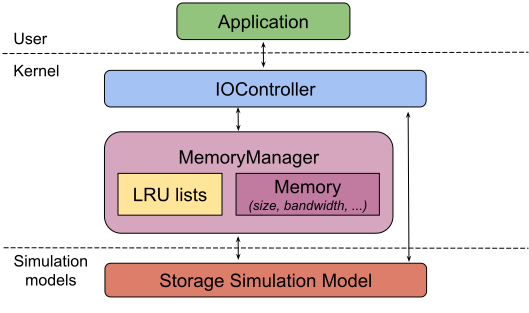
\includegraphics[width=0.85\columnwidth]{figures/interaction.pdf}
           \caption{Overview of the page cache simulator.
           Applications send file read or write requests to the
           IO Controller that orchestrates flushing, eviction, cache
           and disk accesses with the Memory Manager. Concurrent accesses to storage
           devices (memory and disk) are simulated using existing models.}
           \label{fig:interaction}
    \end{figure}

    \subsection{Memory Manager}

    The Memory Manager simulates two parallel threads: the main one
    implements flushing, eviction, and cached I/Os synchronously, whereas
    the second one, operating in the background, periodically searches for
    expired dirty data in page cache LRU lists and flushes them to disk. We
    use existing storage simulation models~\cite{lebre2015} to simulate disk and
    memory, characterized by its storage capacity, read and write
    bandwidths, and latency. Reusing existing storage models allows us to
    simulate bandwidth sharing between concurrent memory accesses and concurrent disk accesses.

    \subsubsection{Page cache LRU lists}

    In the Linux kernel, page cache LRU lists contain file pages. However,
    due to the large number of file pages, managing lists of pages
    induces substantial overheads.
    Therefore, we introduce the concept of a data block as a unit to represent data
    cached in memory. A data block is a subset of file pages stored in
    page cache that were accessed in the same I/O operation.
    A data block has information about file name, block size, last access
    time, a dirty flag that represents whether the data is clean (0)
    or dirty (1), and an entry (creation) time.
    Blocks can have different sizes and a given file can have multiple
    data blocks in page cache. In addition, a data block can be split into an
    arbitrary number of smaller blocks.
    \begin{figure}
           \centering
           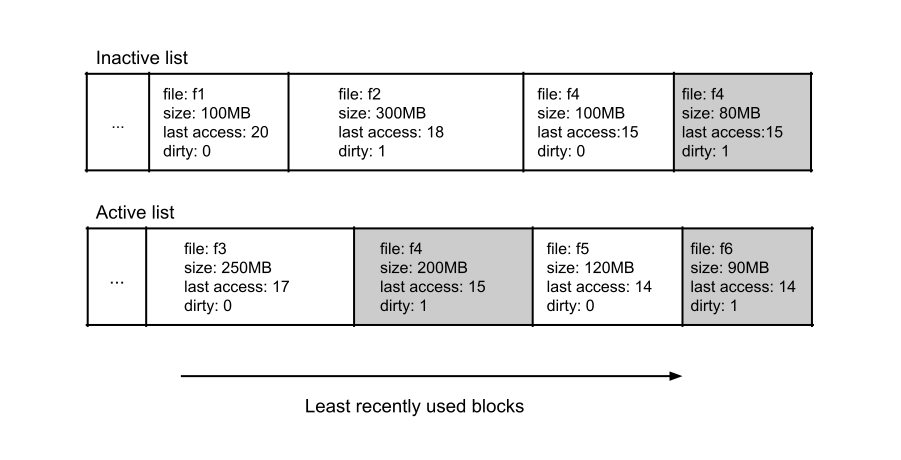
\includegraphics[width=\columnwidth]{figures/lru_lists.pdf}
           \caption{Model of page cache LRU lists with data blocks.}    \label{fig:lrulist}
    \end{figure}

    We model page cache LRU lists as
    two lists of data blocks, an active list and an inactive list, both ordered by
    last access time (earliest first, see Figure~\ref{fig:lrulist}).
    As in the kernel, our simulator limits the size of the active list to
    twice the size of the inactive list, by moving least recently
    used data blocks from the active list to the inactive list~\cite{gorman2004understanding, linuxdev3rd2010}.

    At any given time, a file can be partially cached, completely cached,
    or uncached at all. A cached data block can only reside in one of two
    page cache LRU lists. The first time they are accessed, blocks are
    added to the inactive list. On subsequent accesses, blocks of the
    inactive list are moved to the top of the active list. Cached blocks
    written to cache are marked as dirty until they are flushed to disk.

    \subsubsection{Reads and writes}

    Our simulation model supports chunk-by-chunk file accesses
    with a user-defined chunk size. However, for simplicity, we assume that file pages are
    accessed in a round-robin fashion rather than fully randomly.
    Therefore, when a file is read, cached data is read only after all uncached data was read, and data from the inactive list is read
    before data from the active list
    (data reads occur from left to right in Figure~\ref{fig:read_order}).
    When a chunk of \emph{uncached} data is read, a new clean block is created
    and appended to the inactive list.
    When a chunk of \emph{cached} data is read, one or more existing data blocks in the LRU lists are accessed.
    If these blocks are clean, we merge them together, update the access time and size of the resulting block,
    and append it to the active list.
    If the blocks are dirty, we move them independently to the active list, to preserve their entry time.
    Because the chunk and block sizes may be different, there are situations
    where a block is not entirely read.
    In this case, the block is split in two smaller blocks and one of them is re-accessed.
    % From Tristan: not sure where to put this nor if it's necessary:
    % , in which chunks are read/written
    % until file is entirely read/written.
    \begin{figure}
           \centering
           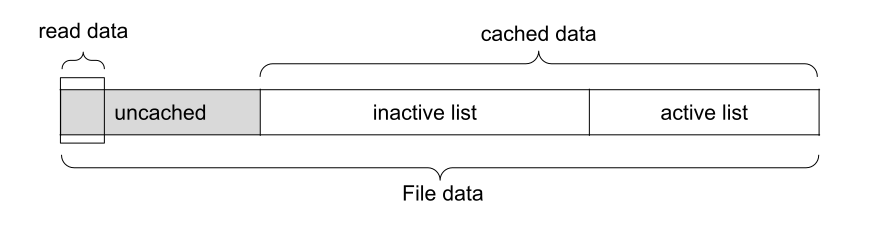
\includegraphics[width=\columnwidth]{figures/read_order.pdf}
           \caption{File data read order. Data is read from left to right: uncached data
           is read first, followed by data from the inactive list, and finally data from the active list. }
           \label{fig:read_order}
    \end{figure}

    For file writes, we assume that all data to be written is
    uncached. Thus, each time a chunk is written, we create a block of dirty data
    and append it to the inactive list.

    \subsubsection{Flushing and eviction}

    The main simulated thread in the Memory Manager can flush or evict data from the
    memory cache. The data flushing simulation
    function takes the amount of data to flush as parameter. While
    the amount of data to flush is not reached and there are dirty
    blocks remaining in cache, this function traverses the sorted
    inactive list, then the sorted active list, and writes the
    least recently used dirty block to disk, having set its dirty
    flag to 0. In case the amount of data to flush requires that a
    block be partially flushed, the block is split in two blocks,
    one that is flushed and one that remains dirty. Flushing time
    to disk is simulated by the storage model.

    The cache eviction simulation also runs in
    the main thread. It frees up the page cache by traversing and deleting
    least recently used clean data blocks in the inactive list.
    The amount of data to evict is passed as a parameter and data blocks are deleted
    from the inactive list until the evicted data reaches the required amount,
    or until there is no clean block left in the list.
    If the last evicted block does not have to be entirely evicted, the block is split in two blocks,
    and only one of them is evicted.
    The cache eviction simulation does not contribute to the simulated time
    since cache eviction time is negligible in real systems \tristan{a reference would be welcome}.

    \begin{algorithm}\caption{Periodical flushing simulation in IO Controller}\label{alg:pdflush}
        \small
        \begin{algorithmic}[1]
            \Input
                \Desc{in}{page cache inactive list}
                \Desc{ac}{page cache active list}
                \Desc{t}{predefined flushing time interval}
                \Desc{exp}{predefined expiration time}
                \Desc{sm}{storage simulation model}
               \EndInput
               \While{host is on}
                \State blocks = expired\_blocks(exp, in) + expired\_blocks(exp, ac)
                \State flushing\_time = sm.write(blocks)
                \State for blk in blocks: blk.dirty = 0
                \If{flushing\_time $<$ t}
                    \State sleep(t - flushing\_time)
                \EndIf  % Else: do nothing, continue the loop
            \EndWhile
        \end{algorithmic}
    \end{algorithm}

    Periodical flushing is simulated in the Memory Manager
    background thread. As in the Linux kernel, a dirty block
    in our model is considered expired if (1) it is dirty, and (2)
    the duration since its entry time is longer than a
    predefined expiration time.
    Periodical flushing is simulated as an infinite loop in which
    the Memory Manager searches and flushes these expired dirty blocks to disk (Algorithm~\ref{alg:pdflush}).
    % From Tristan: the algorithm is quite straightforward, I don't think this is
    % necessary
    % In each repetition, Memory Manager finds expired dirty blocks in two
    % page cache LRU lists (line 8), simulates writes of data of these blocks
    % to disk (line 9), and mark them as clean (line 10).
    % If the flushing time does not exceed our time interval, the thread is put
    % to sleep for the remaining time (lines 11-13).
    % Then based on the state of the host at current simulated time,
    % the algorithm continues or finishes the loop.
    Because periodical flushing is simulated as a background thread, it can happen concurrently
    with disk I/O initiated by the main thread. This is taken into account by the
    storage model and reflected in simulated I/O time.

    \subsection{I/O Controller}

    \begin{algorithm}\caption{File chunk read simulation in IO Controller}
    \label{alg:read}
        \small
        \begin{algorithmic}[1]
            \Input
                \Desc{cs}{chunk size}
                \Desc{fn}{file name}
                \Desc{fs}{file size (assumed to fit in memory)}
                \Desc{mm}{MemoryManager object}
                \Desc{sm}{storage simulation model}
               \EndInput
               \State disk\_read = min(cs, fs - mm.cached(fn)) \Comment{To be read from disk}
               \State cache\_read = cs - disk\_read \Comment{To be read from cache}
               \State required\_mem = cs + disk\_read
               \State mm.flush(cs + disk\_read - mm.free\_mem - mm.evictable, fn)
               \State mm.evict(cs + disk\_read - mm.free\_mem, fn)
               \If {disk\_read $>$ 0}  \Comment{Read uncached data}
               \State sm.read(disk\_read)
               \State mm.add\_to\_cache(disk\_read, fn)
               \EndIf
               \If {cache\_read $>$ 0} \Comment{Read cached}
               \State mm.cache\_read(cache\_read)
            \EndIf
            \State mm.use\_anonymous\_mem(cs)
        \end{algorithmic}
    \end{algorithm}
    As mentioned previously, our model reads and writes file chunks in a
    round-robin fashion. To read a file chunk, simulated applications send
    chunk read requests to the IO Controller which processes them using
    Algorithm~\ref{alg:read}. First, we calculate the amount of uncached
    data that needs to be read from disk, and the remaining amount is read
    from cache (line 6-7). The amount of memory required to read the chunk
    is calculated, corresponding to a copy of the chunk in anonymous memory
    and a copy of the chunk in cache (line 8).
    If there is not enough available memory, the Memory Manager is called
    to flush dirty data (line 9). If necessary, flushing is complemented by
    eviction (line 10). Note that, when called with negative arguments, functions
    \texttt{flush} and \texttt{evict} simply return and do not do anything. Then, if there is
    uncached data, memory manager is called to read data from disk and add this
    data to cache (line 12).
    If cached data needs to be read, the Memory Manager is called to simulate
    a cache read  and update the corresponding data blocks accordingly (line 15).
    Finally, the memory manager is called to reduce the amount of free memory
    corresponding to the amount of anonymous memory used by application (line 17).

    \begin{algorithm}\caption{File chunk write simulation in IO Controller}
    \label{alg:write}
        \small
        \begin{algorithmic}[1]
            \Input
                \Desc{cs}{chunk size}
                \Desc{fn}{file name}
                \Desc{mm}{MemoryManager object}
               \EndInput
            \State remain\_dirty = dirty\_ratio * mm.avail\_mem - mm.dirty
            \If {remain\_dirty $>$ 0} \Comment{Write with memory bandwidth}
                \State mm.evict(min(cs, remain\_dirty) - mm.free\_mem)
                \State mem\_amt = min(cs, mm.free\_mem)
                \State mm.write\_to\_cache(fn, mem\_amt)
            \EndIf
            \State remaining = cs - mem\_amt
            \While {remaining $>$ 0}  \Comment{Write with disk bandwidth}
                \State mm.flush(cs - mem\_amt)
                \State mm.evict(cs - mem\_amt  - mm.free\_mem)
                \State to\_cache = min(remaining, mm.free\_mem)
                \State mm.write\_to\_cache(fn, to\_cache)
                \State remaining = remaining - to\_cache
            \EndWhile

        \end{algorithmic}
    \end{algorithm}
    Algorithm~\ref{alg:write} describes our simulation of chunk writes in
    the IO Controller.
    % Data is written to cache until the amount of dirty data in the cache
    % exceeds the dirty ratio times the amount of available memory. Data is then written to disk.
    Our algorithm initially checks the  amount of data that
    can be written as dirty data given the dirty ratio (line 5).
    If this amount is greater than 0, the Memory Manager is requested to evict
    data from cache if necessary (line 7).
    After eviction, the amount of data that can be written to
    page cache is calculated (line 8), and a cache write is simulated (line 9).
    If there is remaining data, this data is written to cache in a loop (line 12 - line 18).
    In this loop, we flush and evict data as possible so that there will be
    available space for writing (line 13-14).
    After flushing and eviction, the amount of data that can be written
    is calculated (line 15) and a cache write is simulated (line 16).
    We update the remaining amount (line 17) and continue the loop until all data
    is written.

    In addition to the chunk write simulation with writeback page cache above,
    we also add a chunk write function with write-through strategy to the IOController.
    This function simply simulates a disk write with the amount of data passed in,
    then evicts cache if needed and adds this data to cache.

        \subsection{Implementation}

            To validate our simulation model, we created a simple prototype
            simulator independent of existing simulation frameworks and libraries.
            This allowed us to evaluate the accuracy and correctness of our
            model in a simple scenario before integrating it to the more complex
            WRENCH framework.
            In this prototype we used the following basic storage model for
            both memory and disk:
            \begin{align*}
                & t_{r} = D / b_r \\
                & t_{w} = D / b_w\
            \end{align*}

            where:
            \begin{itemize}
                \item $t_{r}$ is the data read time
                \item $t_{w}$ is the data write time
                \item $D$ is the amount of data to read or write
                \item $b_r$ is the read bandwidth of the device
                \item $b_w$ is the write bandwidth of the device
            \end{itemize}

            Since bandwidth sharing was not simulated, this prototype does not support
            concurrency: it is limited to single-threaded applications running on systems
            with a single-core CPU. We used this prototype for a first validation of our simulation
            model against a real sequential application running on a real system.
            The source code this prototype is available at
            \url{https://github.com/big-data-lab-team/paper-io-simulation/tree/master/exp/pysim}. We used Python 3.7.

            We also implemented our model as part of WRENCH, enhancing its internal implementation
            and APIs with a page cache abstraction, and allowing users to activate the feature via a
            command-line argument. For the experiments in this paper we use WRENCH 1.6 at this commit \url{https://github.com/wrench-project/wrench/tree/67185374330d2c4bf274fce222c937e838df5b03}, which uses
            SimGrid 3.25 (available at \url{https://framagit.org/simgrid/simgrid}). However, our implementation is now part of WRENCH's master branch and will be available to users with the next WRENCH release. 

\tristan{anything else interesting to mention about the implementation?}
\henri{I mentioned that the implementaion is now part of the WRENCH master }

        \subsection{Experiments}

        Our experiments compare real executions with our Python prototype,
        with the original WRENCH, and with our WRENCH-cache extension. We
        evaluate our page cache simulation in single-threaded and
        multi-threaded applications, accessing data on local and remote
        file systems.

        We simulate an application that consists of three single-core, sequential tasks
        where each task reads the file produced by the previous task,
        increments every byte of this file to emulate real processing, and
        writes the resulting data to disk.
        In real execution, we clear cache before starting the application to make sure
        the conditions are consistent, the cache is not in use and it is only used by
        our application.
        In addition, the anonymous memory used by application
        is released after each task in the pipeline.
        Thus, we also release the memory used at the end of each task in our simulator.
        We also use a real application
        \textcolor{red}{[Maybe briefly describe this application's purpose
        (e.g. a standard fMRI preprocessing piepeline)]}, to evaluate the
        applicability of our simulation model.

        The real application runs on a dedicated cluster hosted at
        Concordia University, with one login node, 9 compute nodes, and 4
        storage nodes connected with a network bandwidth of 25 Gbps. Each
        compute node has 2 $\times$ 16-core Intel(R) Xeon(R) Gold 6130 CPU
        @ 2.10GHz, 275~GB (256~GiB) \tristan{are you sure it's not 256GB?
        pls check.} of RAM, 6 $\times$ SSDs of 450~GB each with the XFS
        file system, 378~GB of tmpfs, and 126~GB of devtmpfs file system.
        Nodes run CentOS~8.1 with NFS version 4. We use the \texttt{atop}
        and \texttt{collectl} tools to monitor and collect memory status
        and disk throughput.

        To parametrize our simulators, we benchmarked the bandwidths of
        memory, local disk, remote disk (NFS), and network
        (Table~\ref{table:benchmark}). Since SimGrid, and thus WRENCH, currently only supports
        symmetrical bandwidths, we use the mean of the read and write
        bandwidth values in our experiments.
            \begin{table}[htbp]
            \centering
            \begin{tabularx}{\columnwidth}{|l
            |>{\centering\arraybackslash}X
            |>{\centering\arraybackslash}X
            |>{\centering\arraybackslash}X|}
            \hline
                Bandwidths  & Cluster (real) & Python simulator & WRENCH simulator\\
            \hline
                Memory read  & 6860    & 4812     & 4812\\
                Memory write & 2764    & 4812 & 4812\\
                Local disk read & 510 & 465 & 465\\
                Local disk write & 420 & 465     & 465\\
                Remote disk read & 515 & - & 445\\
                Remote disk write & 375 & - & 445\\
                Network & 3000 & - & 3000\\
            \hline
            \end{tabularx}
            \caption{Bandwidth benchmarks (MBps) and simulator configurations.
            The bandwidths used in the simulations are the average of the read and write bandwidths
            measured in the cluster.
            Remote disk and network accesses are not simulated in the Python simulator. \tristan{table could be prettified}}
            \label{table:benchmark}
            \end{table}

            As our focus is on I/O rather than compute, we measured
            application task durations on a cluster node and used these
            durations in our simulation. For the Python simulator,
            execution times were directly used in the simulation. For
            WRENCH and WRENCH-cache, we determined the corresponding number
            of flops on a 1~Gflops CPU and used these values in the
            simulation (see Table~\ref{table:cputime}). The final simulated
            platform and application used in our experiment are avaiable at
            \url{https://github.com/wrench-project/wrench/tree/ec6b43561b95977002258c0fe37a4ecad8f1d33f/examples/basic-examples/io-pagecache}.

            \begin{table}[htbp]
            \centering
            \begin{tabularx}{0.8\columnwidth}{|l|>{\centering\arraybackslash}X|}
            \hline
                Input size (GB)  & CPU time (second)\\
            \hline
                3      & 4.4 \\
                20  & 28 \\
                50  & 75 \\
                75  & 110 \\
                100  & 155 \\
            \hline
            \end{tabularx}
            \caption{Task CPU time corresponding to input file size.}
            \label{table:cputime}
            \end{table}

            % Finally, because WRENCH simulates applications base on network-communication,
            % we use an infinite bandwidth to eliminate network latency for local I/Os.

            Our first experiment (\textit{Exp single-threaded}) simply runs one instance of the
            application on a single cluster node, with different input file
            sizes (20~GB, 50~GB, 75~GB, 100~GB), and with all I/Os directed
            to the same local disk. The goal is to validate the simulation model
            in absence of any concurrent disk access.

            Our second experiment (\textit{Exp concurrent}) runs concurrent instances of the
            application on a single node, all application instances
            operating on different files of size 3~GB stored in the same
            local disk, sharing the disk bandwidth. We vary the number of
            concurrent application instances from 1 to 32 since cluster
            nodes have 32 CPU cores.

            Our third experiment (\textit{Exp NFS}) occurs in the same configuration as the
            previous one, albeit reading and writing on a 400-GB NFS-mounted remote disk
            mounted from another compute node. As is commonly
            configured in HPC environments to avoid data loss, in our simulator,
            NFS client and server read caches are enabled, but there is no cache
            for writing on client side and server writes are configured with
            write-through cache instead of writeback.
            Therefore, all the writes happen at disk bandwidth, but
            reads can benefit from cache hits. We simulate write-through by
            writing data directly to disk and adding that data to the server
            cache.

            Finally, we simulate a real application from the neuroimaging
            domain. \textcolor{red}{[Description of the real pipeline with
            nighres (including the workflow engine if it's Dask)]}.
            We simulate this pipeline with simulators using original WRENCH
            and WRENCH-cache. Because our work focuses on I/O time, we
            assume that CPU time is correctly modeled and use the CPU time
            measured in the real pipelines to setup our simulated
            application.

    \section{Results}
    \label{results}

        \subsection{Single-threaded experiment}

        The page cache simulation model drastically reduces I/O simulation
        errors in the three successive application tasks (Figure~\ref{fig:single_error}). The first read is not impacted
        as it only involves uncached data. Errors are reduced from an average
        of 345\% in the original WRENCH to 46\% in the Python prototype and
        39\% in WRENCH-cache. Unsurprisingly, the original WRENCH simulator
        significantly overestimates read and write times, due to its lack
        of page cache simulation model. Results with files of 50~GB and 75~GBs
        show similar behaviors and are not reported due to space limitations.

        WRENCH simulation errors are substantially lower with 100~GB
        files than with 20~GB files, due to the fact that part of the
        100~GB file needs to be read and written to disk, the only storage
        device in WRENCH, as it does not fit in cache. Conversely,
        simulation errors of the Python prototype and WRENCH-cache are higher with
        100~GB files than with 20~GB files, due to idiosyncracies in the kernel
        flushing and eviction strategies.

        Simulated memory profiles are highly consistent with the real ones
        (Figure~\ref{fig:single_memprof}). With 20~GB files, memory
        profiles almost exactly match the real ones, although dirty data
        seems to be flushing faster in real life than in simulation
        \tristan{any idea why?}, a behavior also observed with 100~GB files. With
        100~GB files, used memory reaches total memory during the first write,
        triggering dirty data flushing. Used memory drops to cached memory
        when application tasks release anonymous memory. Simulated cached
        memory is highly consistent with real values, except toward the end
        of Read 3 where it slightly increases in simulation but not in
        reality \tristan{why?}. As expected, dirty data remains under the
        dirty ratio. The Python prototype and WRENCH-cache exhibit nearly
        identical memory profiles, which reinforces the confidence in our
        implementation.

        The content of the simulated memory cache is also highly consistent
        with reality (Figure~\ref{fig:single_cache}). With 20~GB files, the
        simulated cache content exactly matches reality, owing to the fact
        that all files fit in page cache. With 100~GB files, a slight
        discrepancy is observed after Write 2, which explains the
        simulation error previously mentioned in Read 3. In the real execution indeed,
        File 3 is entirely cached after Write 2, whereas in the simulated execution, part
        of it is on disk. This is due to the fact that the simulated flushing and eviction
        was triggered after File 3 was already written, while in reality these operations
        happened before File 3 was written \tristan{Dzung, pls check that. Also, why doesn't it happen irl?}.

        % We conclude from this experiment that our model can accurately
        % simulate cached I/Os in a sequential context. The next experiment
        % evaluates our simulation with concurrent I/Os.

            \begin{figure*}
            \centering
            \begin{subfigure}{\linewidth}
                \centering
                   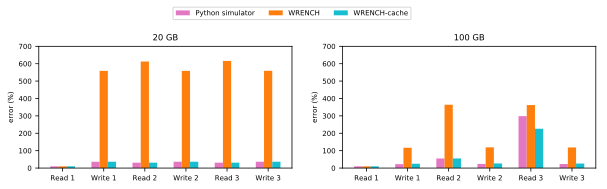
\includegraphics[width=\linewidth]{result/single/figures/single_errors.pdf}
                   \vspace*{-0.7cm}
                   \caption{Absolute relative simulation errors}
                   \vspace*{0.5cm}
                   \label{fig:single_error}
                \end{subfigure}
            \begin{subfigure}{\linewidth}
                \centering
                %    Gray shades represent task phases (read, compute and write).
                %    Lines represent memory usage along pipeline execution time.}
                   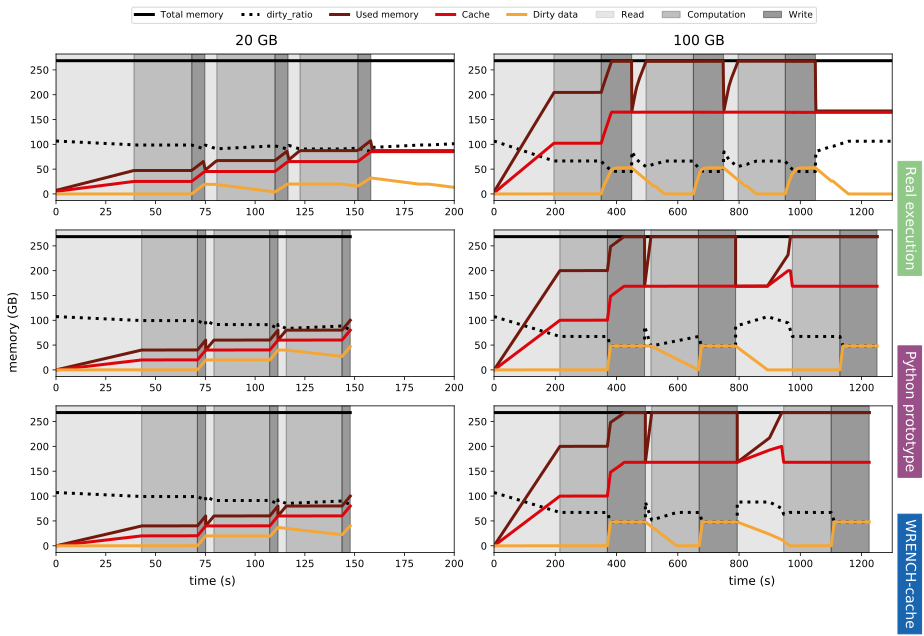
\includegraphics[width=\linewidth]{result/single/figures/single_memprof.pdf}
                   \vspace*{-0.7cm}
                   \caption{Memory profiles \tristan{Remove trailing whitespace for 20GB graphs (xmax should be about 160s, not 200s)}}
                   \vspace*{0.5cm}
                   \label{fig:single_memprof}
            \end{subfigure}
            \begin{subfigure}{\linewidth}
                \centering
                   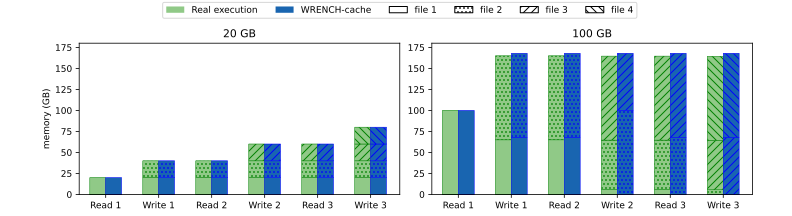
\includegraphics[width=1.05\linewidth]{result/single/figures/cached_files.pdf}
                   \caption{Cache contents \emph{after} application I/O operations}
                %    \textcolor{red}{Update real results of 20GB}}
                   \label{fig:single_cache}
            \end{subfigure}
            \caption{Single-threaded results}
            \end{figure*}



        \subsection{Concurrent applications}

            \begin{figure*}
            \begin{subfigure}{\linewidth}
                \centering
                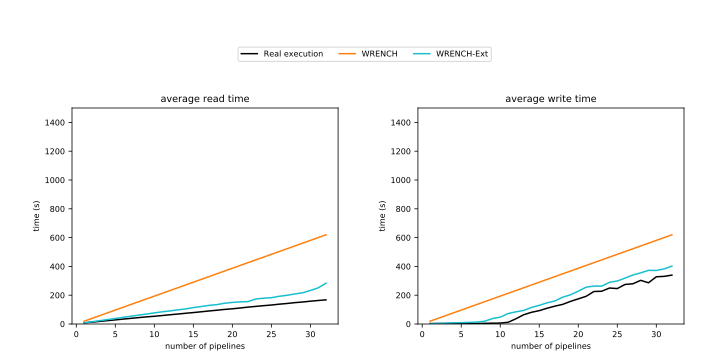
\includegraphics[width=\linewidth]{result/multi/figures/multi_local.pdf}
            \end{subfigure}
            \caption{Concurrent results with 3~GB files (averages on 5 repetitions)}
            \label{fig:multi_local}
            \end{figure*}

            The page cache model notably reduce WRENCH's simulation error
            for concurrent applications and local I/Os
            (Figure~\ref{fig:multi_local}). For reads, WRENCH-cache still
            slightly overestimates reality, due to the discrepancy between
            simulated and real read bandwidths mentioned before
            (\tristan{check it's indeed mentioned. Dzung: is it correct?}). For writes,
            WRENCH-cache slightly underestimates reality for the same reason. The plateau
            ending around 7 concurrent pipelines in the WRENCH-cache curve
            marks the limit beyond which the page cache is saturated with dirty data
            and needs flushing \tristan{why is there no plateay irl?}.

        \subsection{Remote storage}

            \begin{figure*}
            \begin{subfigure}{\linewidth}
                \centering
                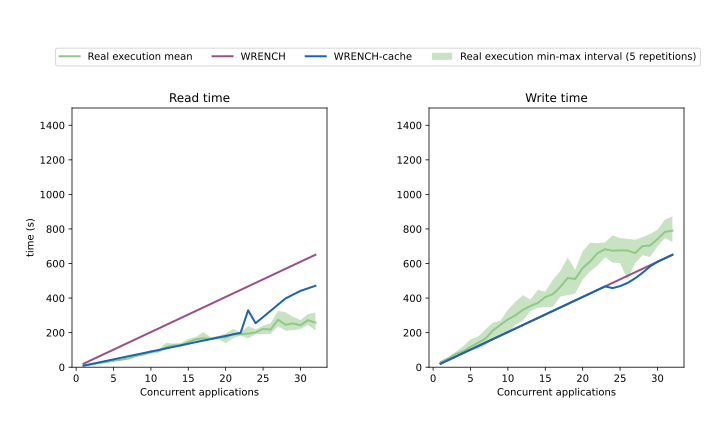
\includegraphics[width=\linewidth]{result/multi/figures/multi_nfs.pdf}
            \end{subfigure}
            \caption{NFS results with 3~GB files (averages on 5 repetitions)}
            \label{fig:multi_nfs}
            \end{figure*}

            Page cache simulation importantly reduces the simulation error
            on remote storage as well (Figure~\ref{fig:multi_nfs}). This
            manifests only for reads, as only write-through cache was
            enabled in the NFS server. Both WRENCH and WRENCH-cache
            underestimate write times due to the discrepancy between
            simulated and real bandwidths mentioned previously. For reads,
            this discrepancy only impacts the results beyond 22
            applications since before this threshold, most reads result in cache
            hits \tristan{Dzung, pls check that.}.

        \subsection{Real application}
        \subsection{Overhead comparison}
        \tristan{Dzung, add your overhead measures here.}

    \section{Conclusion}
    \label{discussion}
        Page cache undoubtedly has important impacts on performance, in
        particular for data-intensive applications. Numerical simulation is
        an effective approach to predict and compare the performance of
        applications, schedulers and infrastructures. However, page cache
        is missing in many simulation tools for distributed systems. In
        this study, we proposed a simulation model of I/Os with page cache,
        we implemented it in the SimGrid-based WRENCH library, and we
        evaluated its benefits in different conditions. Results show that
        our model very substantially improves simulation accuracy,
        decreasing absolute relative errors between simulated and real
        performance by a factor close to 10 (see results of the
        single-threaded experiment). Furthermore, this level of accuracy
        can be achieved without a fine-grained level of details
        \tristan{not sure what you mean}. Our page cache model is available
        in WRENCH from commit \tristan{abcd}, ready to be used for the
        simulation of Big Data applications.

        Simulation results could be made even more accurate by a deeper
        investigation of cache eviction mechanisms \tristan{be more
        specific}. The availability of asymmetrical bandwidths in the
        forthcoming SimGrid release will also directly improve our
        simulation accuracy. Relevant future work includes simulating
        application memory consumption, random I/O, file readahead and
        persistent disk storage.

        \tristan{discussion could be fleshed out}

        \section{Acknowledgments}
The computing platform used in the experiments was obtained with funding
from the Canada Foundation for Innovation.

\bibliographystyle{IEEEtran}
\tristan{Check references, in particular capitalization}
\bibliography{citation}

\end{document}
